{$\space$\par}
\vspace{0.5cm}
\justifying
\section*{{\bfseries \LARGE Questão 3 -} {\bfseries \large Represente a separação entre esses alunos em um plano bidimensional.}}

\vspace{0.3cm}

\textcolor{red}{Uma maneira de representar a separação dos alunos em relação ao espaço dos parâmetros em dimensões menores é computar a matriz de distâncias no espaço dos parâmetros e então usá-la para projetar em dimensões menores.
Primeiro, normalizei as quantidades de diferentes colunas para uma melhor comparação entre o CRA, média no ENEM e o ano de ingresso. Então, calculei a matriz de distância e projetei em 2 dimensões.}

\vspace{0.4cm}

\begin{lstlisting}
# Distance matrix
m_dist = dist(scale(astro[,c(2:8)]))

# Projecting on 2 dim
projected = cmdscale(m_dist)

# Plots
plot(projected[,1], projected[,2], cex=2,col='red',
pch=16,xlab='Projecao 1', ylab="Projecao 2", cex.lab=2)
text(projected[,1], projected[,2],
     labels = astro$Nome,
     pos = 3,    
     cex = 1.5)
\end{lstlisting}

\begin{figure}[h]
    \centering
    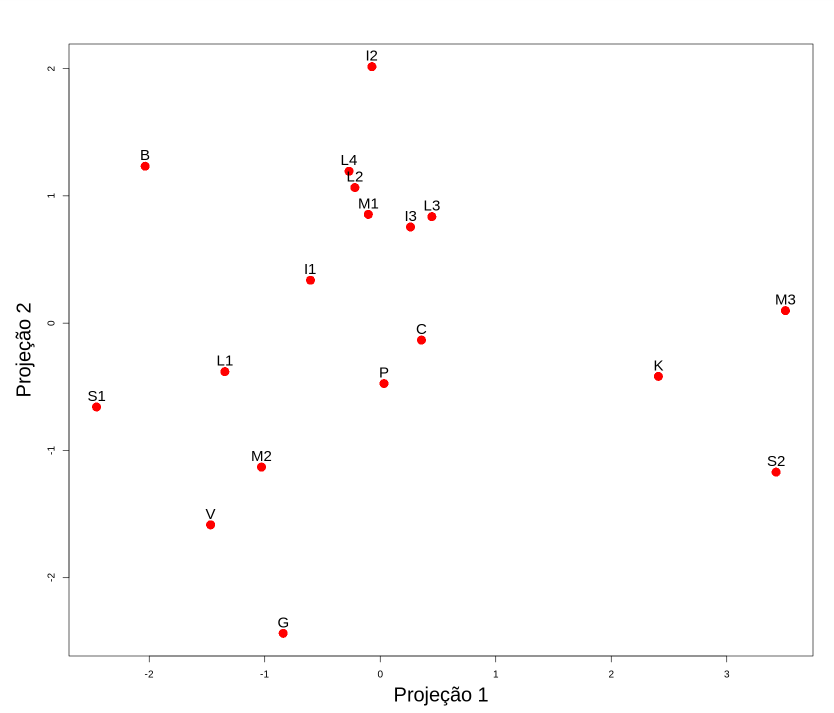
\includegraphics[width=0.6\linewidth]{Figuras/projected.png}
    \caption{Projeção do espaço de parâmetro dos alunos em 2 dimensões com o respectivo nome acima.}
    \label{projected}
\end{figure}